
Die folgende Tabelle zeigt die Ergebnisse
der Optimierung der Testfunktionen
mit Variablenbeschr�nkung, wobei die Minimalstellen
immer noch in dem zul�ssigen Bereich bleiben.

\begin{table}[h]
\centering
\begin{tabular*}{0.5\linewidth}{@{\extracolsep{\fill}}lcc}
  \toprule
  Problem &   SSN   &   SQP   \\
  \cmidrule{2-3}
          & \multicolumn{2}{c}{T (ms)} \\
  \midrule
  Rosenbrock     &  16.72  &  25.62  \\
  Himmelblau     &  17.34  &  30.31  \\
  Bazaraa-Shetty &  53.59  & 109.38  \\
  Colville       & 593.75  & 656.25  \\
  \bottomrule
\end{tabular*}
\caption{Vergleich}
\end{table}

\begin{testproblem}
\emph{(Lineare Regression, vgl. Beispiel 1.1.6 in \cite[S.~4f]{alt})}\\
Gegeben seien m-Messwerte $(\xi_i,\eta_i), i = 1,\ldots,m$.
Gesucht ist eine Gerade
\begin{equation}
  \eta(\xi) := x_1 \xi + x_2,
\end{equation}
die ``optimal'' zu den Messwerten passt.
D.\,h. wir sollen den Parameter $x = (x_1,x_2)^T \in \R^2$
so bestimmen, dass die Summe der Fehlerquadrate
in den Messpunkten minimiert wird.
Dazu definieren wir die Zielfunktion durch
\begin{equation}
  f(x) := \sum_{i=1}^{m} (\eta(\xi_i) - \eta_i)^2
        = \sum_{i=1}^{m} (x_1 \xi_i + x_2 - \eta_i)^2.
\end{equation}
Es ist damit ein unrestringiertes Optimierungsproblem zu l�sen.
\end{testproblem}

\begin{testproblem}
\emph{(Nichtlineare Regression, vgl. Abschnitt 2.3.2 in \cite[S.~30f]{alt})}\\
Neben linearen Regressionsaufgaben sind auch oft
nichtlineare Regressionsaufgaben zu l�sen.
Gesucht sind den funktionalen Zusammenhang $\eta(\xi)$
zwischen den $\xi$- und den $\eta$-Werten,
beispielweise
\begin{equation}
  \eta(\xi) := x_1 e^{\xi x_2} + x_3.
\end{equation}
Dabei ist $x = (x_1,\ldots,x_n)^T \in \R^n$ ein Parametervektor, der optimal
bestimmt werden soll.
\end{testproblem}

\begin{table}[h]
\centering
\begin{tabular*}{0.8\linewidth}{@{\extracolsep{\fill}}c|cccccccccc}
  %\toprule
  $\xi_i$ & 1 & 2 & 3 & 4 & 5 & 6 & 7 & 8 & 9 & 10 \\
  \midrule
  $\eta_i$ & 1 & 1.1 & 1.2 & 1.35 & 1.55
    & 1.75 & 2.5 & 3 & 3.7 & 4.5 \\
  %\bottomrule
\end{tabular*}
\caption{Gegebene Messwerte}
\end{table}

\begin{table}[h]
\centering
\begin{tabular*}{0.8\linewidth}{@{\extracolsep{\fill}}c|cccccccccc}
  %\toprule
  $\xi_i$ & 1 & 2 & 3 & 4 & 5 & 6 & 7 & 8 & 9 & 10 \\
  \midrule
  $\eta_i$ & $-\frac{1}{2}$ & $-2$ & $-3$ & $-3$ & $-2\frac{1}{2}$
    & $-2$ & $-1$ & 1 & 3 & $5\frac{1}{2}$ \\
  %\bottomrule
\end{tabular*}
\caption{Gegebene Messwerte}
\end{table}

\begin{figure}[ht]
\centering
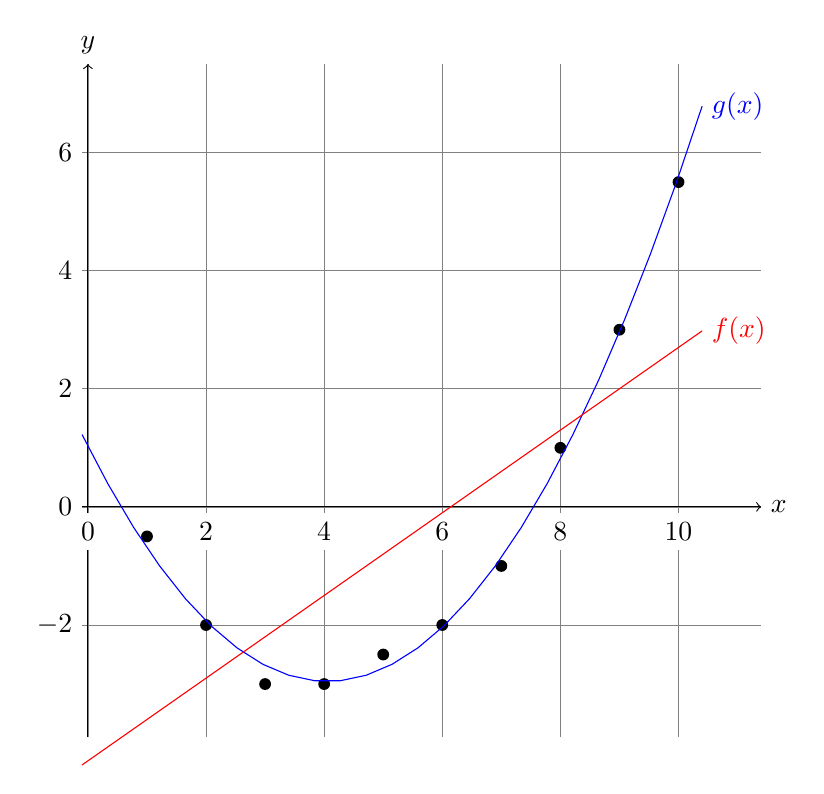
\begin{tikzpicture}[domain=-0.1:10.4,scale=0.75]
  \draw[very thin,color=gray,step=2] (-0.1,-3.9) grid (11.4,7.5);
  \draw[->] (-0.1,0) -- (11.4,0) node[right] {$x$};
  \draw[->] (0,-3.9) -- (0,7.5) node[above] {$y$};
  %\draw (-0.1,0.2) node [below left,fill=white] {0};
  \foreach \x in {0,2,4,...,10}
    \draw (\x,-0.1) node[below,fill=white] {$\x$};
  \foreach \y in {-2,0,2,4,6}
    \draw (-0.1,\y) node[left] {$\y$};
  \foreach \x/\y in
    {1/-0.5, 2/-2, 3/-3, 4/-3, 5/-2.5, 6/-2, 7/-1, 8/1, 9/3, 10/5.5}
    \fill (\x,\y) circle(0.1);
  \draw[color=blue] plot (\x,{0.242*(\x-4.056)^2-2.955}) node[right] {$g(x)$};
  \draw[color=red] plot (\x,{0.7*\x-4.3}) node[right] {$f(x)$};
\end{tikzpicture}
\caption{$f(x) = 0.7 x - 4.3
  \text{ und } g(x) = 0.242 (x - 4.056)^2 - 2.955$}
\end{figure}


\begin{testproblem}
L�se folgendes, einfaches, 2-dimensionales Problem.
\begin{align}
  \min_{x \in \R^2}\ (x_1 - 1)^2 + (x_2 &- 2.5)^2 \\
  \nb -x_1 + 2x_2 & \leq 2 \\
       x_1 + 2x_2 & \leq 6 \\
       x_1 - 2x_2 & \leq 6 \\
                0 & \leq x_1, x_2
\end{align}
\end{testproblem}

\begin{figure}[ht]
\centering
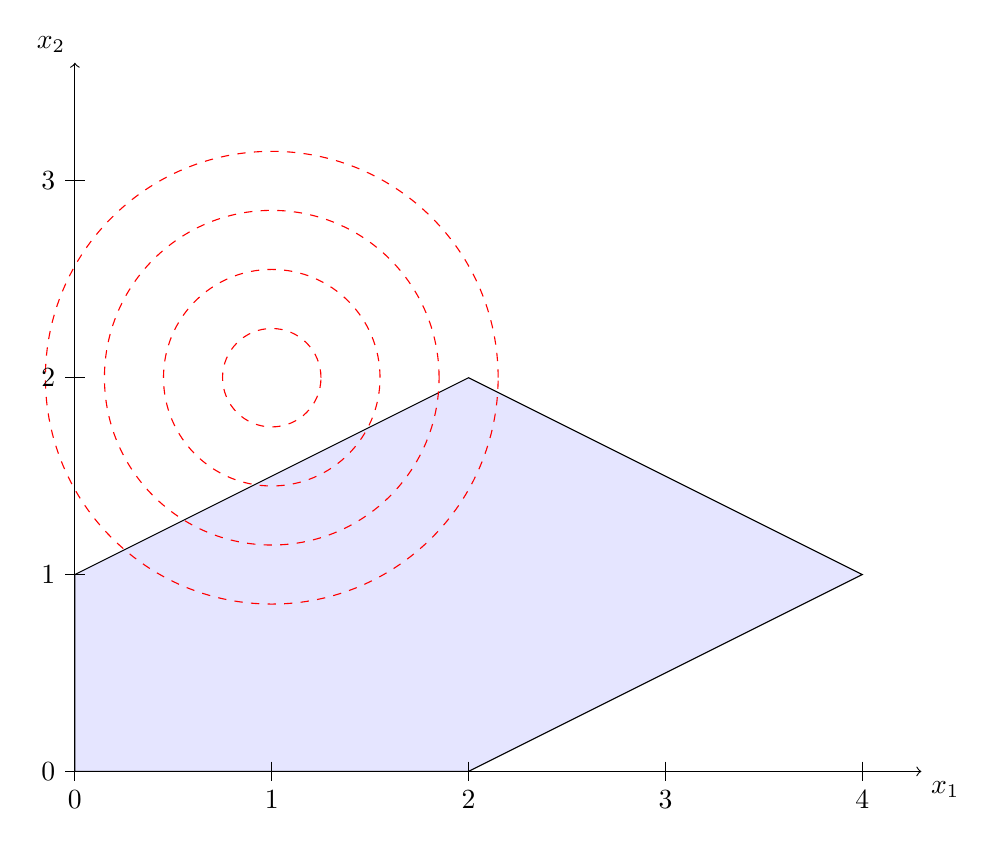
\begin{tikzpicture}[scale=2.5]
  
  % Die zul�ssige Menge
  \draw[fill=blue!10] (0,0) -- (0,1) -- (2,2) -- (4,1) -- (2,0) -- cycle;
  \draw (1.7,1) node {$\F$};
  
  % Die Niveaulinien
  \foreach \r in {0.25, 0.55, 0.85, 1.15}
    \draw[dashed,color=red] (1,2) circle (\r);
  
  % Koordinatenachsen
  \draw[->] (0,0) -- (4.3,0) node [below right] {$x_1$};
  \foreach \x in {0,...,4}
    \draw (\x,0.05) -- (\x,-0.05) node [below] {\x};
  \draw[->] (0,0) -- (0,3.6) node [above left] {$x_2$};
  \foreach \y in {0,...,3}
    \draw (0.05,\y) -- (-0.05,\y) node [left] {\y};
  
\end{tikzpicture}
\caption{Restringiertes Problem}
\end{figure}
